\chapter{Introduction to space debris and observations}\label{chap:introduction}

The term space debris encompasses all artificial non-functional objects orbiting around Earth. Each object has different physical properties, such as size and shape and is made of different materials which determine its behaviour and ease of tracking. Usually, in literature, space debris is categorized into four different groups by its type:
\begin{enumerate}
	\item mission-related debris,
	\item fragmentation debris,
	\item non-functional spacecraft,
	\item rocket bodies.
\end{enumerate}

	Despite having many different sources and causes, the clearest line is drawn between debris released intentionally and unintentionally. Examples of the former are launch adapters, lens covers, and many other components associated with launch events and payload deployment. The latter category contains protective gloves, cooling liquids, or small particles released from material decay (Klinkrad, 2006). Common feature of all these objects is that it’s referred to as mission-related debris as well because it’s result of a spacecraft’s deployment, activation or operation.
	
	The polar opposite of mission-related debris is fragmentation debris. As the name indicates, it’s objects or particles created during destructive disassociation of a rocket body or an orbital payload and as a result of deterioration when smaller-than-the-parent-object fragments are created. Breakups may be intentional or accidental and are the largest portion of catalogued orbital debris. Products of breakups are ejected into the surrounding area in toroidal cloud with various initial velocities and spread until they reach the limit of maximum inclination and altitudes of the debris (UN, 1999?).
	
	Another commonly mentioned type of space debris in various literature is non-functional spacecraft. First deployed man-made satellite was Sputnik-1 on October 4, 1957. As of January 2017, there have been 5253 launches of human-made objects into space since then (ESA, 2017). Even though not all of them were satellites, they still are a common source of breakup events and the following creation of orbital debris. However, a satellite doesn’t have to break into smaller pieces to be considered debris. Functional spacecrafts that reach their end of life are either re-orbited or left in their former orbit. Historically, re-orbiting manoeuvres were performed only in GEO orbit and by spacecrafts carrying nuclear material in LEO orbit, as well as for vehicles with crew and for reconnaissance. Nevertheless, according to the Mitigation Guidelines released in 2002 by Inter-Agency Space Debris Coordination Committee (IADC), spacecrafts in LEO should be allowed to fall into the atmosphere and burn up within 25 years of mission end and spacecrafts in GEO should be re-orbited at least 300 kilometres above the GEO orbital ring and left in so-called “graveyard orbit”. Satellites in GEO are not lowered because it’s not efficient to carry extra fuel specifically for this purpose.
	
	The last category of orbital debris consists of rocket bodies. Spacecrafts which are placed into orbit for their missions are launched on vehicles which are constructed for this single purpose. Deployment process has one or more stages that are represented by rocket bodies. The number of rocket bodies needed for ascent into desired altitude is proportional to the altitude – for example spacecrafts with missions in LEO only need one rocket body while those in GEO need may need up to three. First stages need to have enough thrust to lift the satellite despite gravity and air resistance and are generally bigger than other stages which are used to position the spacecraft in the final steps of deployment. As such, larger rocket bodies usually re-enter into the atmosphere and burn up or fall into the ocean, while the smaller stages are left at various altitudes. This kind of space debris poses danger especially because of its large dimensions and potentially leftover fuel that may cause explosions.
	
\subsection{Small space debris}\label{subsec:small_space_debris}
The size of space debris varies from particles less than one millimetre small to objects more than one metre large. While the smallest particles are difficult to track, the amount of those that have size less than 1 centimetre is estimated to be more than 170 million (ESA, 2017). Other sources list the population of debris with diameters bigger than 1 mm as $3*10^8$ objects and $3*101^3$ objects with diameter bigger than 1 µm (Klinkrad, 2006). 

	A major source of sub-centimetre reproductive space debris is the effect of harsh space environment on spacecraft surface materials. Intense UV radiation and atomic oxygen cause decay on spacecraft surfaces which is usually coated in paint for thermal purposes, or other thermal protection materials. Erosion is enhanced through transits through the Earth shadow, when the temperature shifts and the material expands and shrinks. Paint flakes, such as one in Figure \ref{fig:paintflakes}, created by these processes have small initial velocity and in combination with their relatively small size are not as dangerous to functional satellites though they can cause significant damage. They are categorised as fragmentation or sometimes as anomalous debris.
	
\begin{figure}[H]
  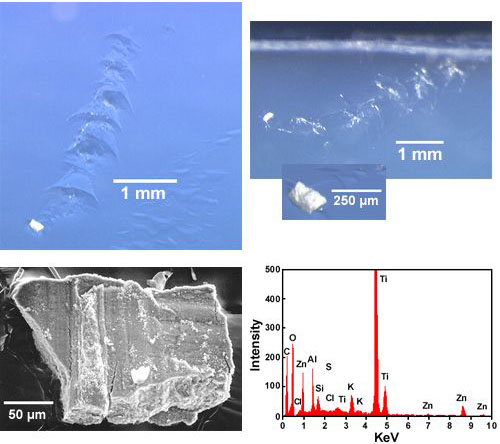
\includegraphics[width=\linewidth]{images/paintflakes}
  \caption{Paint flakes captured by Mir Environmental Effects Payload}
  \label{fig:paintflakes}
\end{figure}
	
	Hypervelocity collisions of small debris objects create particles upon impact which are called ejecta and are part of the fragmentation debris group. When assessing the number of small particles, it’s important to acknowledge small meteoroids as well. This type of debris is not detectable from ground and is measured by examining surfaces of spacecrafts returned to Earth or by dedicated debris detectors situated in LEO altitudes. The most successful method for this is chemical analysis of impact craters. However, because of the mentioned high speeds of many of these particles, the pressure under which the impact is made is more than 100 GPa and temperatures more than 9000 degrees Celsius (Klinkrad, 2006). As a result of this there is only a little impacting material left on the surface since most of it evaporates. Another important attribute which can be deduced from impact craters, though not easily, is size of the impactor.  On the other hand, time and position of spacecraft in orbit is almost impossible to determine from impact craters. Figure \ref{fig:hypervelocitycollision} shows a hypervelocity impact which created a hole in a panel of the Solar Maximum Mission satellite.
	
\begin{figure}[H]
  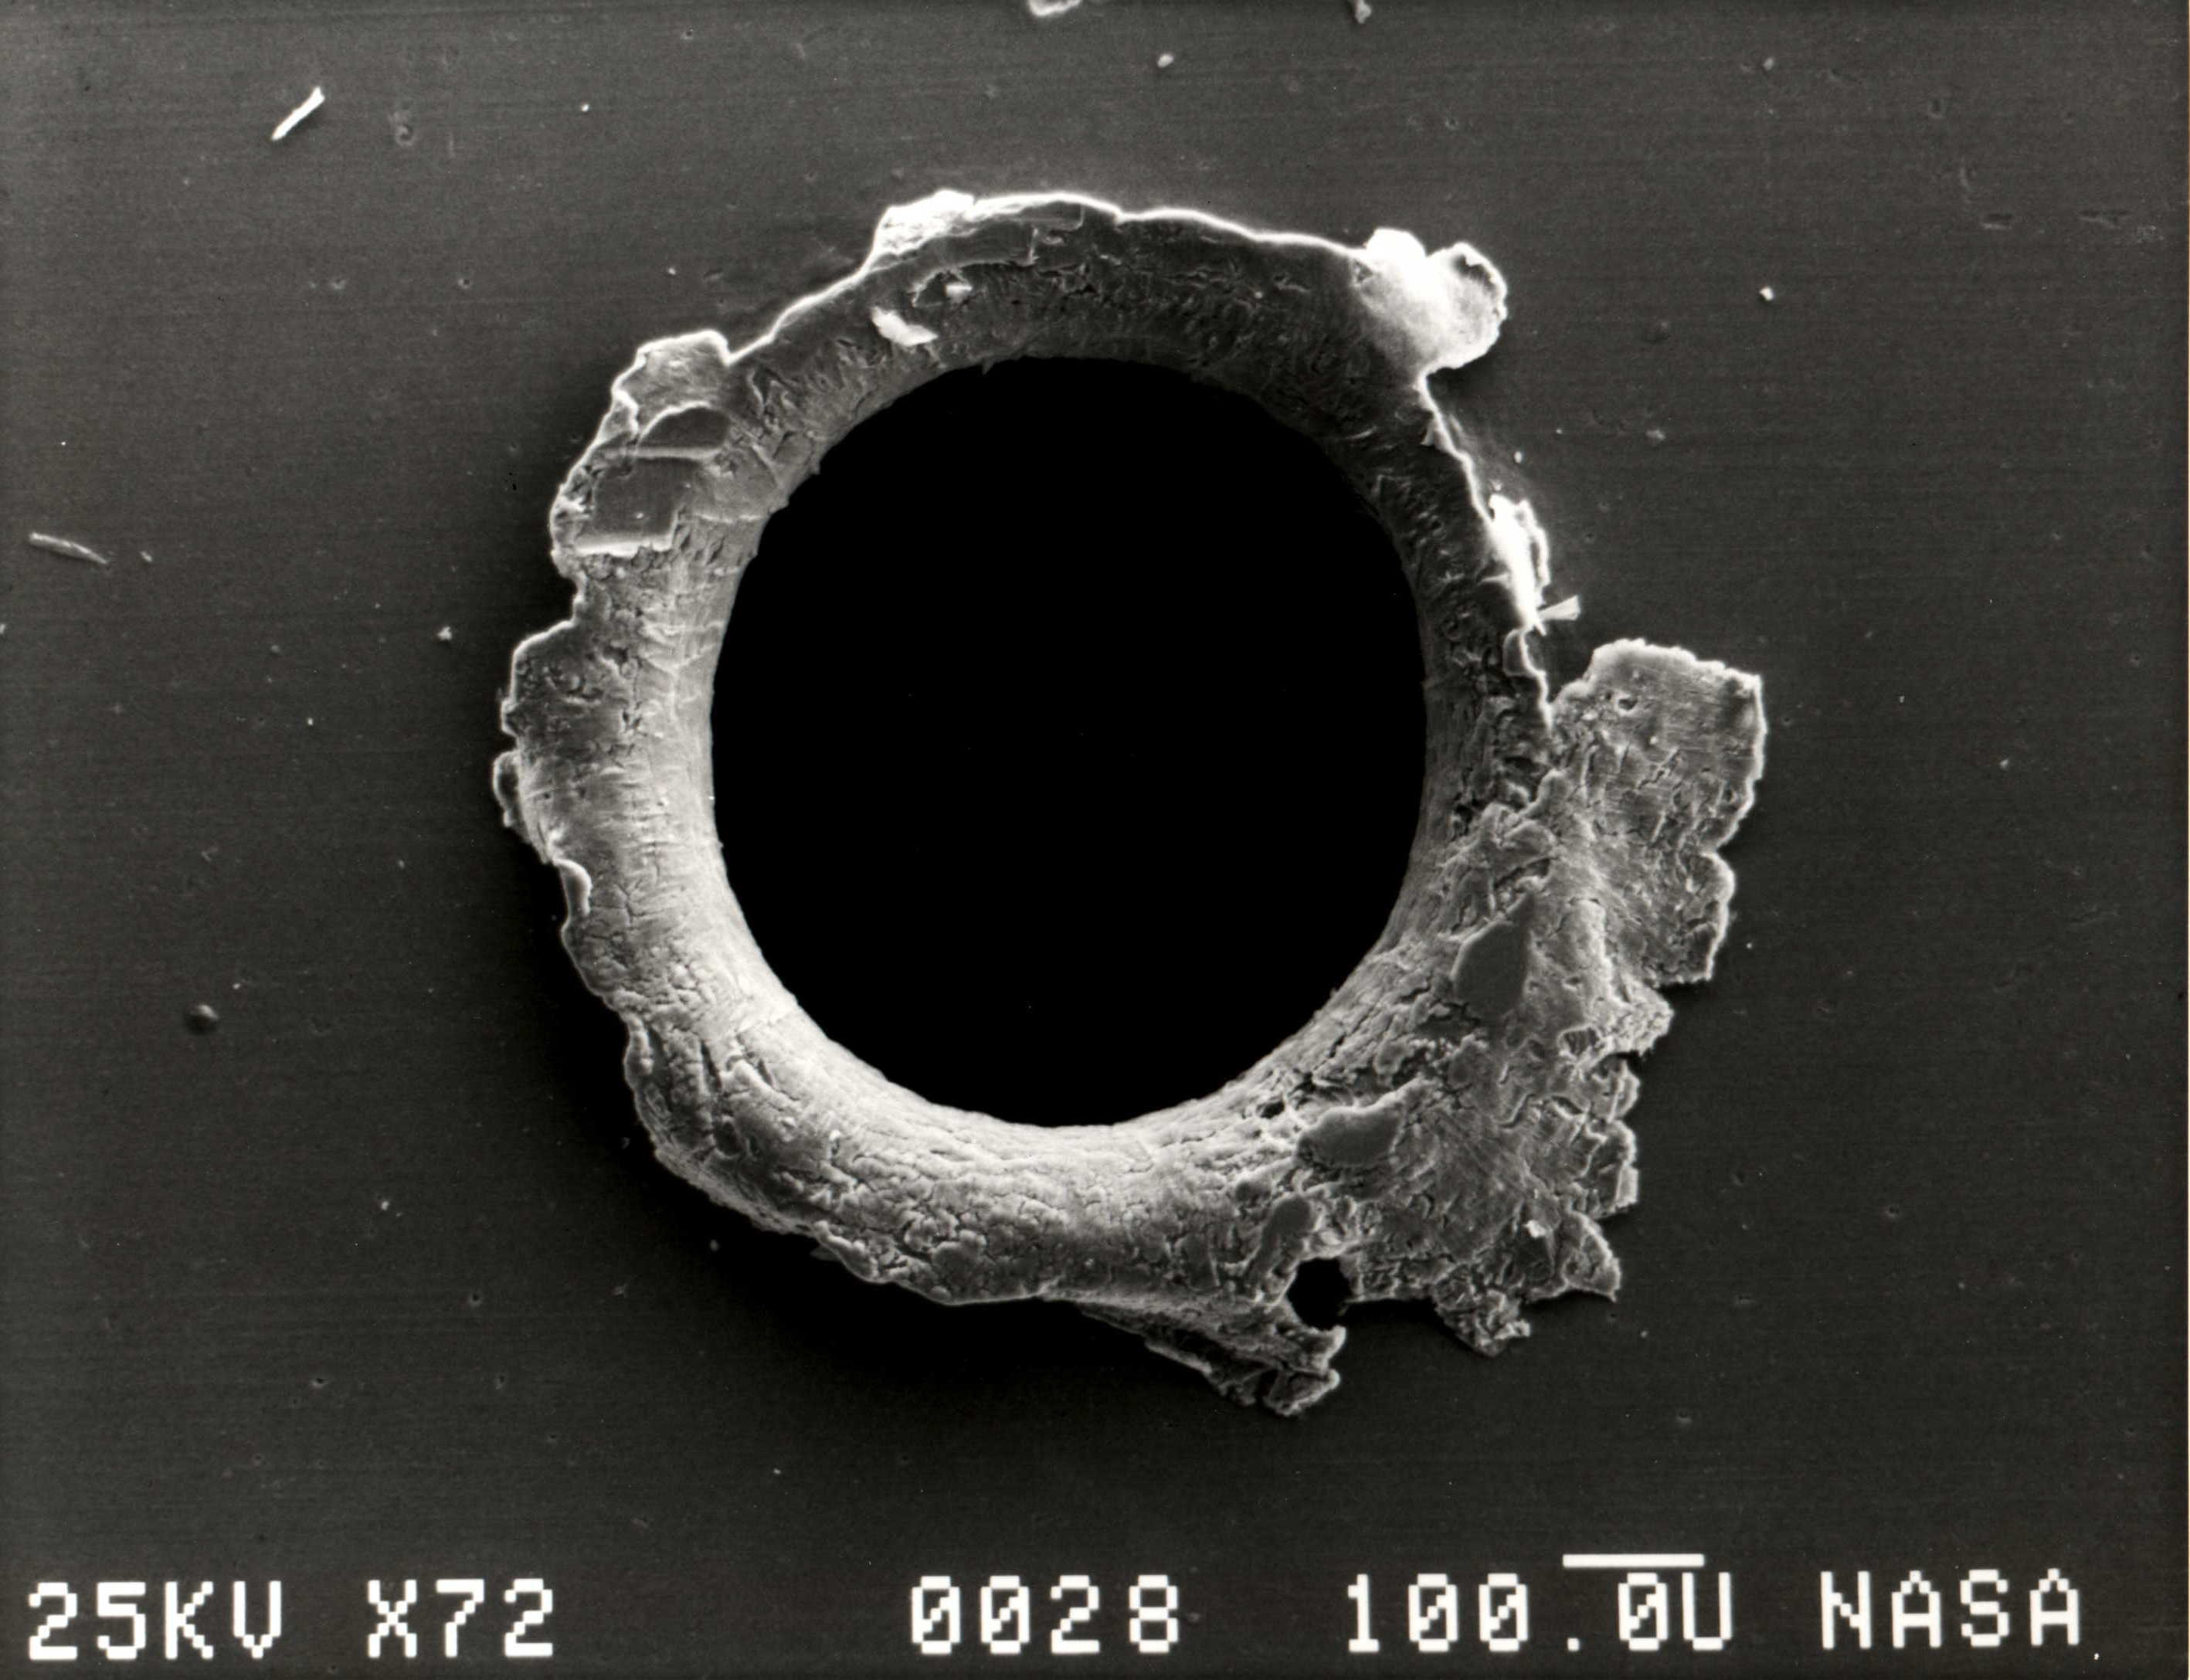
\includegraphics[width=\linewidth]{images/hypervelocitycollision}
  \caption{A hole made by debris in a solar panel}
  \label{fig:hypervelocitycollision}
\end{figure}	
	
	While delivering payloads into orbit, burning process of solid rocket motors releases particles called SRM slag and SRM dust which are classified as non-fragmentation, unintentional debris and are composed mainly of aluminium oxide. The aim of adding aluminium to most solid fuels is to stabilize the combustion process. SRM slag is fused during the main thrust phase from trapped aluminium oxide, melted aluminium droplets and thermal insulation liner material. Their sizes are between 0.1 and 30 mm. It is assumed that during 1032 SRM firings throughout 44 years, or 2440 up to year 2017 (ESA, 2017), about 1000 tons of propellant were released, 320 of them were aluminium oxide particles (SRM dust) and 4 tons SRM slag. Due to orbital perturbations and different sizes, it is estimated that only 1 ton of SRM dust and 3 tons of SRM slag remain in the orbit (Klinkrad, 2006). Figure \ref{fig:srmslag} shows a piece of SRM slag recovered from a test firing of a shuttle solid rocket booster.
	
\begin{figure}[H]
  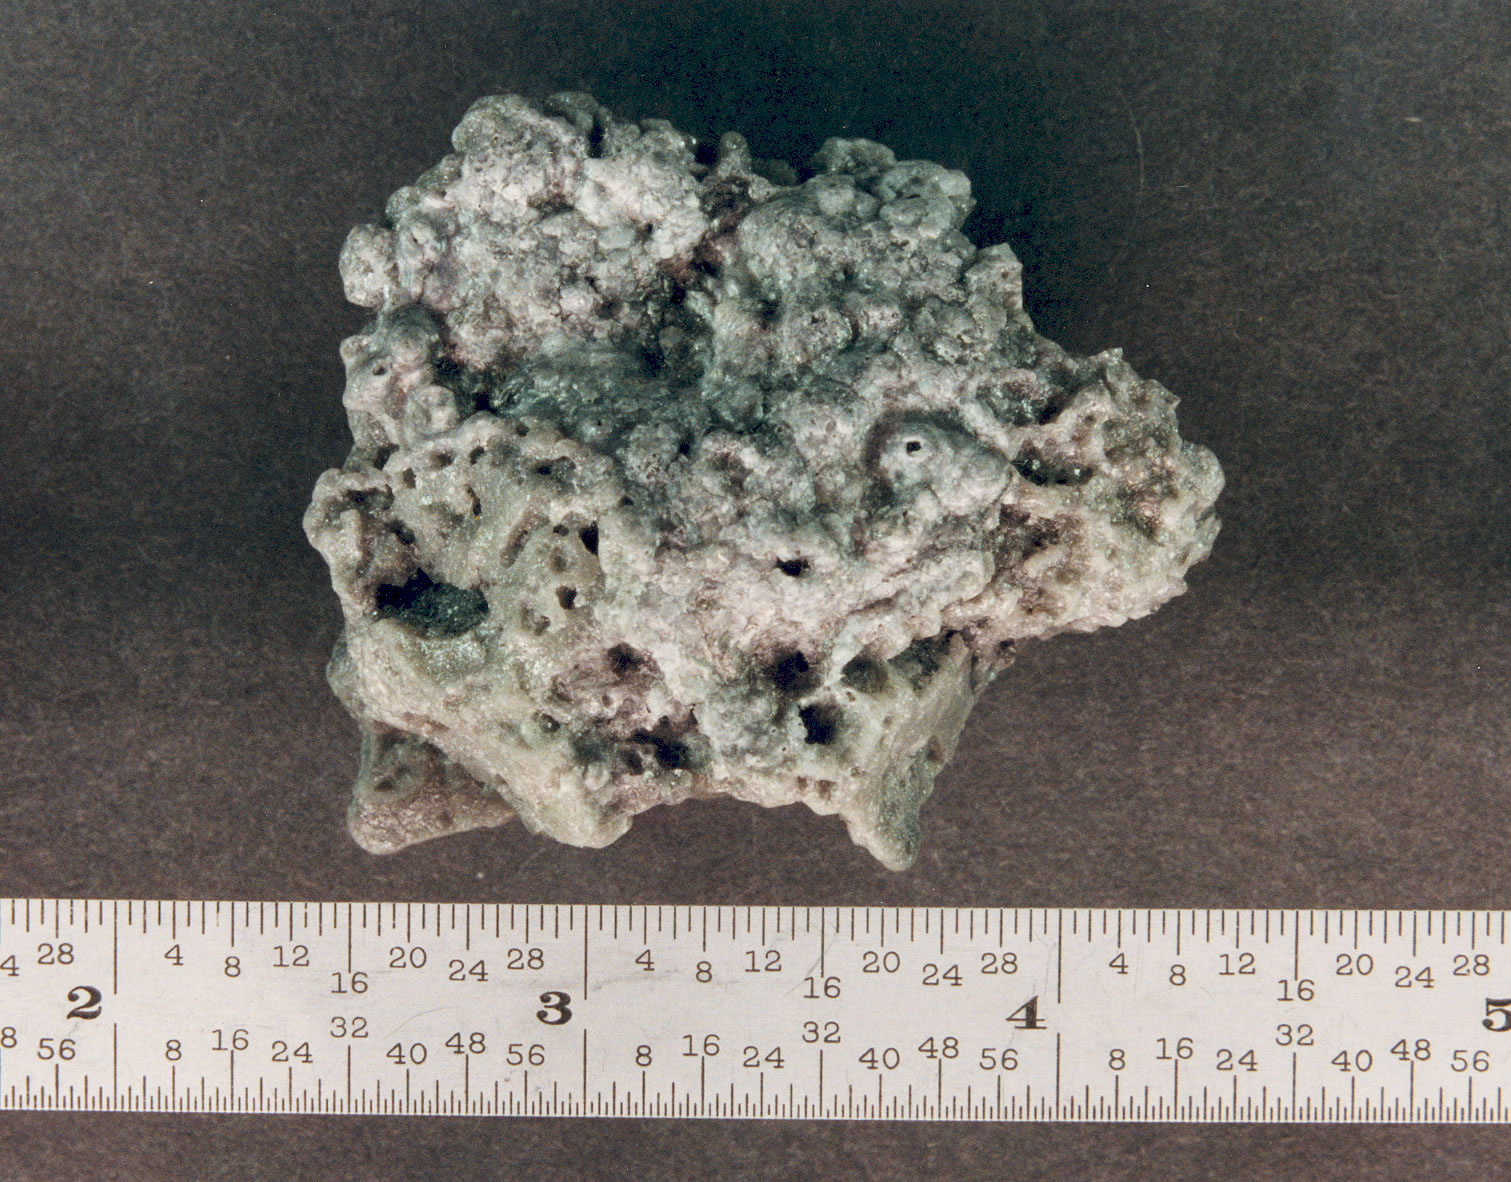
\includegraphics[width=\linewidth]{images/slag}
  \caption{SRM slag}
  \label{fig:srmslag}
\end{figure}	
	
	Another similar but rare type is droplets of sodium-potassium alloy (NaK), a coolant in Russian RORSAT (Radar Ocean Reconnaissance Satellites¬). To the contrary to previous methods used to capture and observe small debris, these particles were detected by ground-based radar and optical measurements in the early 1990s. NaK droplets were used in a particular type of reactor used between October 1970 and March 1988, throughout sixteen launch events. It is estimated that whole of 208 kilograms of NaK coolant was released during this period. However, smaller droplets evaporate due to thermodynamics which puts this type of debris to an estimated mass of 50 to 60 kilograms. Since this kind of reactor is no longer used, NaK droplets along with Westford Needles are considered a historic, non-reproducing space debris. 
	
	A communications experiment between years 1961 and 1963 consisted of deploying copper wires around the Earth. These copper wires were 1.78 cm long and 25.4 $\mu$m in diameter in the first experiment and 17.8 $\mu$m in diameter in the second experiment - see Figure \ref{fig:westfordneedles}. They were originally encased in rotating containers and supposed to disperse to form a layer of radio frequency reflecting diploes. However, the dispersion failed, and the estimated mass of Westford Needles is less than 60 kg in two clusters, first being 40 000 in needles and the second 1000.
	
\begin{figure}[H]
  
\includegraphics[width=\linewidth]{images/westfordneedles}
  \caption{Westford needles}
  \label{fig:westfordneedles}
\end{figure}	
	
	
	While being the major contributor to the population of space debris, small objects are, as mentioned, virtually unobservable from the ground, only by radars and space-based telescopes positioned on LEO, and therefore are not the main focus of this work.

\subsection{Large space debris}\label{subsec:large_space_debris}
The most extensive database of tracked objects in orbit is maintained by US Space Surveillance Network (USSSN). As mentioned above, only objects which exceed certain sizes at certain altitudes can be tracked with ground-based radar and optical measurements. Due to this, USSSN incorporates only debris larger than five to ten centimetres in LEO and thirty centimetres to one metre in GEO (geostationary altitudes, approximately 36000 kilometres). Currently, USSSN contains more than 42 thousand tracked objects with more than half of them still in orbit. About 24\% of them are satellites and 18\% are spent upper stages and other mission-related objects (ESA, 2017). Out of 175 fragmentation events recorded since 1961 until January 2002, 48 have been categorized as deliberate explosions or collisions, 52 as propulsion system explosions, 10 have been caused by aerodynamic forces, 7 are believed to have been electrical system failures and 1 was an accidental collision (Klinkrad, 2006). 

	Deliberate collisions have been caused mainly as test scenarios for Strategic Defence Initiative (SDI) experiment. In the first case, an anti-satellite missile was fired and destroyed Solwind P78-1 satellite. The second collision was between the USA-19 spacecraft and an upper stage used to bring it into the orbit. Number of fragments for both of these events was 285 and 13 respectively but as a result of natural cleaning processes or deliberate planning, from H-10 event only 33 objects were on orbit by January 2002 and from Solwind P78-1 only 2. However, the largest fragmentation event occurred in 2007 when China intentionally destroyed its non-functional weather satellite Fengyun-1C, generating more than 3215 new fragments. 
	
	Even though unintentional collisions are rare and only 0.2\% of all catalogued objects until February 2009 have been created in this way it is expected that they will be a major cause for debris in the future. On November 13, 1986 an Ariane-1 H-10 upper stage exploded, causing a fragment cloud containing 488 catalogue entries. The first unintentional in-orbit collision came to pass 10 years later between a French satellite and the mentioned H-10 upper stage explosion fragment. The Cerise satellite was still able to function afterwards and the event caused only one new piece of debris (Silha, 2012). 
	
	A particularly interesting class of space debris is anomalous debris. It’s a specific group that has small velocity and high area to mass ratio (A/M) and its formation process is unknown. The exemplary member of anomalous debris is multilayer insulation (MLI), and sometimes paint flakes. MLI is used as thermal protection to decrease thermal noise on antennae and satellite buses of spacecrafts. MLI can be divided into two types based on their purpose – as a cover and outer layer, and as a reflector and inner layer.
	
	The rapid creation of new debris of non-negligible sizes is a major concern due to the phenomenon called “Kessler syndrome”. The term was coined in 1978 and it means that “each collision would produce several hundred objects large enough to catalogue, increasing the rate that future collision breakups would occur, resulting in an exponential growth in the collision rate and debris population” (Kessler, 2009). 
	
	Spent upper stages and non-functional satellites are one of the largest and most compact space debris. Even though many of them re-enter the Earth's atmosphere on purpose, or are elevated on further orbits and their life on orbit is relatively short, they still pose a threat to functional satellites or missions in progress. Figure \ref{fig:upperstage} shows such spent upper stage, specifically Agena D, the most launched American upper stage (Genesis of Agena D, 2006).
	
\begin{figure}[H]
  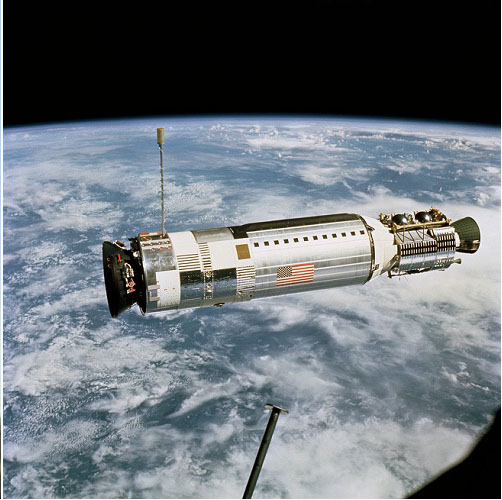
\includegraphics[width=\linewidth]{images/upperstage}
  \caption{Agena D upper stage}
  \label{fig:upperstage}
\end{figure}
	
\pagebreak


\section{Observations and telescopes}\label{sec:observations_telescopes}

Optical telescopes are usually placed at high altitudes, with minimal light pollution and good meteorological and atmospheric conditions. Telescopes used for satellite tracking must be operated at "astronomical night" (Sun being more than 18° under the horizon) while the tracked objects must still be illuminated by the Sun (Klinkrad, 2006).

	Telescopes are divided into two groups: refractors and reflectors. The first type uses lens systems to observe objects while the second one uses mirror surfaces to focus incoming light. Reflectors are categorized into four subgroups:
	
\begin{enumerate}
	\item Newton telescopes,
	\item Cassegrain telescopes,
	\item Coudé telescopes,
	\item Ritchey-Chrétien telescopes.
\end{enumerate}
	
	The base upon which a telescope is placed is called a mount. As with telescopes, there are many types of mounts with each giving different advantages than the other. Mounts are able to rotate both vertically and horizontally.
	
	A telescope collects photons which are reflected or emitted by a space object. Usually, the origin of photons is the Sun and depending on the angle between the Sun, the object and the observer and reflection efficiency of the target the intensity is determined. The light is then translated into an image which can be viewed by an eyepiece or used to generate an exposure on an Charge-Coupled device (CCD). CCDs are photosensitive and solid-state imaging sensors which convert incoming photons into electric charges on an array of photodetectors. The time-tagged information coming from the photodetectors can be reconstructed into an image with a resolution depending on the granularity of the CCD. High-end systems use CCD which produce images with resolution of up to 4096 x 8192 pixels. CCDs naturally heat up and the danger of thermal noise corruption is mitigated by using active coolants, such as liquid nitrogen (Klinkrad, 2006).

\subsection{ESA OGS}\label{subsec:esa_ogs}
European Space Agency (ESA) Optical Ground Station (OGS) is a Zeiss telescope built in the Teide Observatory, in Tenerife, Spain, 2400 m above sea level. It’s a one-metre telescope with focal length 13.3 m originally used for tests with laser link, space debris observation and other astronomical night observations. The CCD camera has a field of 4000 x 4000 pixels. The telescope can detect and track near-GEO objects down to 10-15 cm in size and has photometric observations capabilities and therefore can determine material properties of unknown objects and provides information on origin of newly detected fragments. Throughout years 2009 to 2013 the telescope has been credited by Minor Planet Center (MPC) with discovery of 38 minor planets.
 
	Besides being used for mentioned astronomical purposes, its unique location and ability to be tilted to near-horizontal position and point at a different station, namely Jacobus Kapteyn Telescope in La Palma, allows it to be employed in quantum telecommunication experiments. In 2012 a group of researchers funded by ESA successfully transferred physical properties of one particle to another 143 km away via quantum teleportation. The telescope is currently operated by Instituto de Astrofísica de Canarias (IAC).

	Figure \ref{fig:esaogs1} shows the schematic of ESA OGS. One of the most important parts is the Cassegrain focus where the CCD camera is used for observation of asteroids and for long-term monitoring of comets.


\begin{figure}[H]
  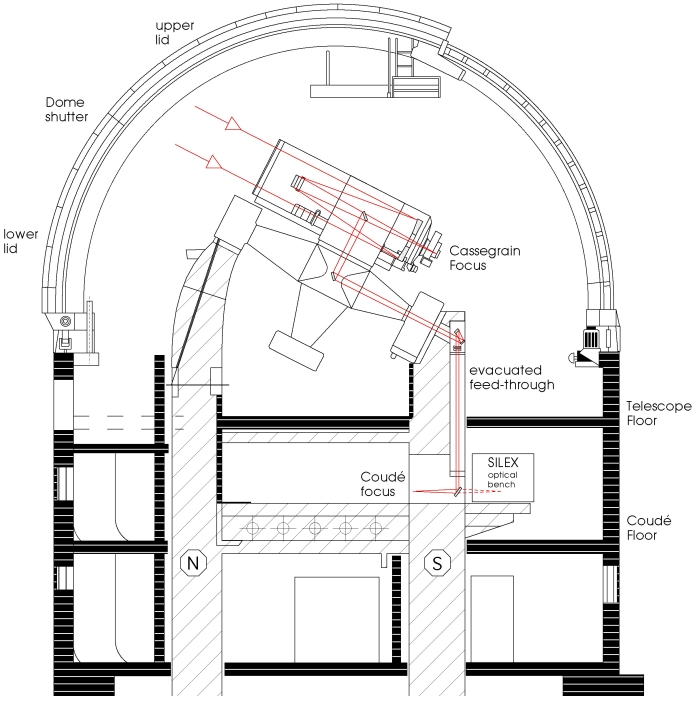
\includegraphics[width=\linewidth]{images/ESAOGS1}
  \caption{ESA OGS schematic}
  \label{fig:esaogs1}
\end{figure}

	Figure \ref{fig:esaogs2} is an image of the Zeiss telescope on the English mount.

\begin{figure}[H]
  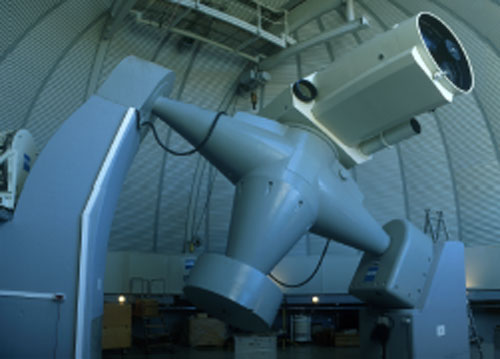
\includegraphics[width=\linewidth]{images/ESAOGS2}
  \caption{ESA OGS telescope}
  \label{fig:esaogs2}
\end{figure}

\subsection{FMPI AGO}\label{subsec:fmpi_ago}
Astronomické a geofyzikálne observatórium (Astronomical and geophysical observatory, or AGO) is located in Modra, Slovakia and belongs to Fakulta matematiky, fyziky a informatiky (Faculty of mathematics, physics and informatics of Comenius University, or FMPI). The observatory has a main reflector telescope with a 0.6m Zeiss telescope with focal length of 3.28m. The CCD camera has resolution of 1024 x 1024 pixels.

	Figure \ref{fig:fmpiago1} shows the main telescope which is operated by a computer.

\begin{figure}[H]
  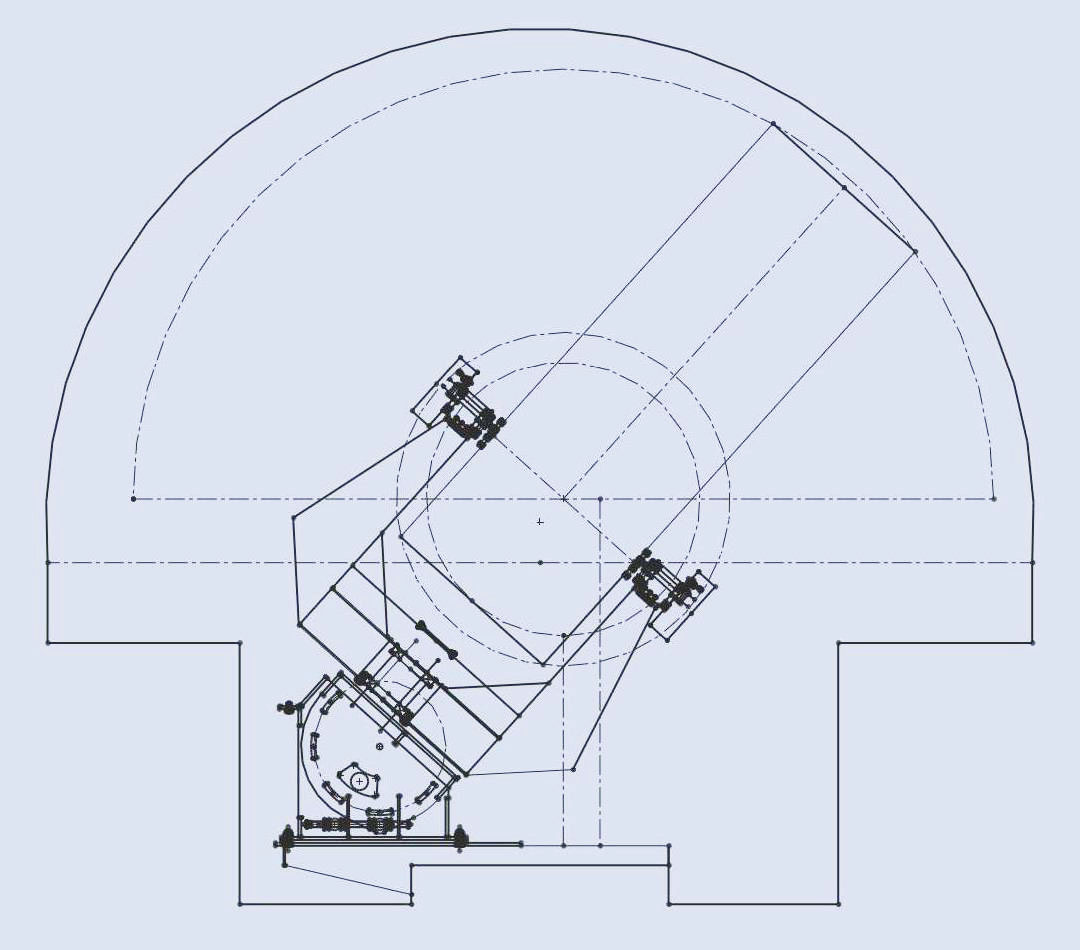
\includegraphics[width=\linewidth]{images/FMPIAGO1}
  \caption{The main Zeiss telescope}
  \label{fig:fmpiago1}
\end{figure}